\chapter{Implementation}

In this chapter we describe how the design of Chapter~\ref{ch:project} is realized in
code: the platform and language, the resulting project structure, the choices made while
implementing the protocol that were not fixed by the requirements, and the implementation
details of the protocol that were deliberately left out of the previous chapter.

\section{Platform}

The system is implemented in Gleam\footnote{https://gleam.run} 1.17, a statically typed
functional language that compiles to the Erlang Virtual Machine (BEAM) and interoperates
with OTP (\texttt{gleam\_otp} 1.2, \texttt{gleam\_erlang} 1.3). This choice follows
directly from the algorithm's own model: one asynchronous process per network node,
communicating only through message passing, with no shared state. This is precisely the
actor model natively provided by the BEAM.

\section{Project structure}

\begin{figure}[htbp]
\centering
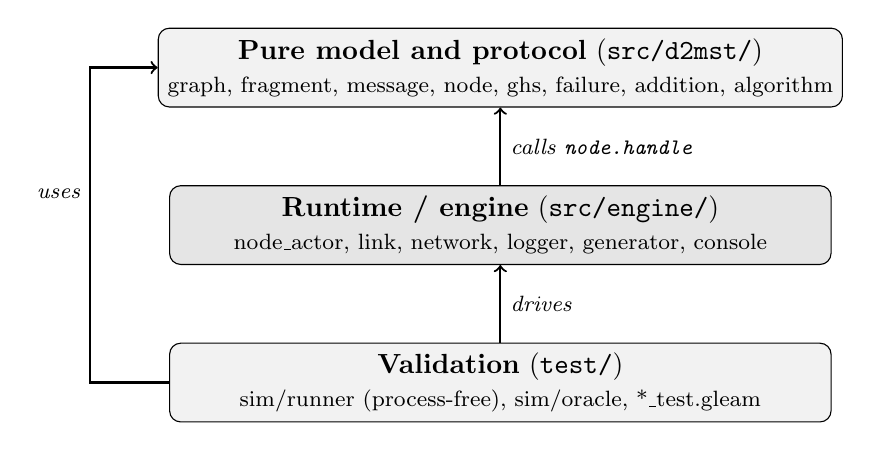
\begin{tikzpicture}[
    box/.style={draw, rounded corners, minimum width=8.4cm, minimum height=1cm, align=center},
    lbl/.style={font=\footnotesize\itshape}
]
\node[box, fill=black!5] (protocol) at (0,4) {\textbf{Pure model and protocol} (\texttt{src/d2mst/})\\
\footnotesize graph, fragment, message, node, ghs, failure, addition, algorithm};
\node[box, fill=black!10] (engine) at (0,2) {\textbf{Runtime / engine} (\texttt{src/engine/})\\
\footnotesize node\_actor, link, network, logger, generator, console};
\node[box, fill=black!5] (test) at (0,0) {\textbf{Validation} (\texttt{test/})\\
\footnotesize sim/runner (process-free), sim/oracle, *\_test.gleam};

\draw[->, thick] (test) -- node[right, lbl] {drives} (engine);
\draw[->, thick] (test.west) -- ++(-1,0) |- node[pos=0.3, left, lbl, align=right] {uses} (protocol.west);
\draw[->, thick] (engine) -- node[right, lbl] {calls \texttt{node.handle}} (protocol);
\end{tikzpicture}
\caption{The three-layer split. Protocol code has no notion of processes; the engine is
the only layer that touches them; validation exercises both, either directly or through
the process-free simulator.}
\label{fig:layers}
\end{figure}

The codebase follows the three-layer split of Figure~\ref{fig:layers}. This separation is
chosen so that the protocol, the part of the system whose correctness matters most, can be
understood, tested, and reasoned about independently of processes, scheduling, or message
loss.

\subsection{Pure model and protocol (\texttt{src/d2mst/})}

Every module in this layer is a pure function of its inputs; none of them import
\texttt{gleam/erlang/process} or \texttt{gleam/otp/actor}.

\begin{itemize}
  \item \texttt{graph.gleam}: the \texttt{Graph}, \texttt{Edge}, and symmetric
  \texttt{EdgeId(low, high)} types, together with \texttt{compare\_edge}, the
  lexicographic order on $(w(e), \mathrm{id}(e))$ that makes the MST unique regardless of
  weight collisions. This order is what allows \texttt{kruskal}, a plain union-find MST
  also defined here, to serve as an exact oracle for the distributed result.
  \item \texttt{fragment.gleam}: the \texttt{FragmentId} type (Section~\ref{sec:fragment-id}).
  \item \texttt{message.gleam}: every wire message, split into \texttt{GHSMsg} (Tier 1),
  \texttt{D2MMsg} (failure response), and \texttt{AddMsg} (addition response), together
  with the two predicates that decide which messages must carry a matching fragment
  identity to be accepted (Section~\ref{sec:intra-fragment}).
  \item \texttt{node.gleam}: the \texttt{State} record, the \texttt{Event} type
  (\texttt{Wakeup}, \texttt{Receive}, \texttt{LinkUp}, \texttt{LinkDown}), the
  \texttt{Effect} type (\texttt{Send}), and small pure helpers shared by every protocol
  module, such as looking up an edge, selecting the minimum edge satisfying a predicate,
  or deferring a message. It contains no protocol logic of its own.
  \item \texttt{ghs.gleam}, \texttt{failure.gleam}, and \texttt{addition.gleam}: the three
  protocol tiers, one module each, all operating on the same \texttt{node.State}. This
  split keeps Tier 1, 2, and 3 almost separated while letting them share state and the
  fragment-identity invariant that makes their concurrent execution safe.
  \item \texttt{algorithm.gleam}: the single exposed entry point,
  \texttt{handle(state, event) -> \#(state, effects)}. It dispatches an event to the
  appropriate tier according to the message type, and then drains the pending queue: a
  message a handler could not yet process (Section~\ref{sec:defer}) is retried after every
  subsequent event, repeatedly, until a pass makes no further progress.
\end{itemize}

\subsection{Runtime / engine (\texttt{src/engine/})} \label{sec:link-actor}

This is the only layer that touches BEAM processes, and the only place where protocol code
is driven by something other than a direct function call.

\begin{itemize}
  \item \texttt{node\_actor.gleam}: a thin actor shell, one BEAM process per graph node.
  It turns every incoming event, whether a wakeup, a received message, or a link
  appearing or disappearing, into a call to \texttt{algorithm.handle}, performs the
  returned \texttt{Send} effects by forwarding them to link actors, and reports every send
  and every resulting state to the logger. It contains no protocol logic of its own.
  \item \texttt{link.gleam}: one actor per edge, so that the process itself represents the
  edge. The system therefore has no separate representation of a failed link: deleting an
  edge means terminating this process directly, and both endpoint nodes, which monitor it,
  observe the termination as an ordinary \texttt{LinkDown} event. A link additionally
  monitors both of its endpoint nodes and stops itself as soon as either one dies, since a
  channel with only one live endpoint no longer serves any purpose. This single rule is
  what reduces a node crash to plain link failures at every neighbor, without any protocol
  code having to distinguish a peer node dying from the edge itself failing.
  \item \texttt{network.gleam}: builds a running network of node and link actors from a
  \texttt{Graph} and exposes the topology-event API used by the tests and the demo:
  \texttt{wake\_all}, \texttt{fail\_link}, \texttt{add\_link}, \texttt{crash\_node}, and
  \texttt{add\_node}. Each of these mutates the live actors and returns an updated
  \texttt{Network} whose \texttt{.graph} field reflects the new topology, so that
  assertions in the tests always compare against the graph that is actually running.
  \item \texttt{logger.gleam}: a central observer process that nodes report to on every
  state change. The protocol never depends on
  it, since it holds no protocol state of its own, only an ordered history that nodes push
  into, and its process is unlinked from the rest of the system, so that killing it does not take the network down with it.
  \item \texttt{generator.gleam}: a seeded generator and a
  connected-graph builder. It is used instead of Erlang's \texttt{:rand} specifically so
  that a failing random test, or a bad round of the interactive demo, is reproducible from
  its integer seed alone. It is also what \texttt{d2mst.gleam} uses to build graphs and to
  schedule random topology events from user-supplied counts.
  \item \texttt{console.gleam}: A thin standard-input and clock wrapper from Erlang code.
\end{itemize}

\subsection{Validation (\texttt{test/})}

\begin{itemize}
  \item \texttt{test/sim/runner.gleam}: a second, process-free runtime. A single FIFO
  queue of \texttt{\#(NodeId, Event)} drives \texttt{algorithm.handle} for every node
  until the system quiesces, all within one BEAM process. It runs the exact same protocol
  modules as the production code, only the driving loop differs, but it is deterministic
  and can be stepped one event at a time, which makes it the preferred tool for chasing a
  logic bug: a failure found here reproduces every time, with no scheduling
  nondeterminism to contend with.
  \item \texttt{test/sim/oracle.gleam}: checks a converged run against
  \texttt{graph.kruskal}. The union of reported tree edges must equal the unique MST,
  there must be exactly one root per connected component, and every parent pointer must be
  a tree edge.
  \item \texttt{test/*\_test.gleam}: Specific unit tests for the modules, and fuzz tests that drive the process-free simulator with random topology events and check the result against the oracle.
\end{itemize}

\section{Decisions made to implement the protocol}

\paragraph{Incremental construction on top of GHS.}
The implementation was built in two stages: GHS (Tier 1) first, then the dynamic
repair protocol on top of it. The dynamic protocol
needs an already-converged spanning tree to operate on, so GHS is kept in the final
system as the mechanism that constructs that initial tree, rather than being replaced
once Tier 2/3 were implemented. One consequence of this ordering is that failure and
addition events are only ever injected once GHS has converged and the tree is stable;
the two protocols were not tested interacting \emph{while} the initial tree is still
being constructed.

\paragraph{Process per edge.}
The design already calls for one logical process per network node. The implementation
takes the same idea further and gives every edge its own process as well
(Section~\ref{sec:link-actor}), rather than having node processes exchange messages
directly. As a consequence, a link failure and a node crash reduce to the same primitive
event, namely a monitored process terminating, observed from different places. The
protocol therefore only ever has to handle one case, \texttt{LinkDown}, and the
failure-transparency requirement of Chapter~\ref{ch:analysis} follows from the runtime
topology rather than requiring dedicated detection code.

\paragraph{Pure state machine.}
Every protocol handler has the shape \texttt{State -> Event -> \#(State, List(Effect))},
with \texttt{Effect} restricted to \texttt{Send(on, msg)}: no module in
\texttt{src/d2mst/} performs I/O, spawns a process, or blocks. \texttt{node\_actor.gleam}
is the only place where an \texttt{Effect} is turned into an actual message send. This
separation is what makes the process-free simulator possible: it links against the same
protocol modules and simply interprets the returned effects into its own event queue
instead of onto real links, so that a bug reproduced in the simulator is necessarily a bug
in the deployed protocol.

\paragraph{MOE search strategy selection.}
Chapter~\ref{ch:project} describes two independent Phase 3 procedures. In the
implementation they are a single type, \texttt{MoeStrategy} (\texttt{Naive} or
\texttt{BinarySearch(sample\_k)}), fixed once per node at \texttt{init} and threaded
through \texttt{failure.gleam}'s \texttt{start\_repair\_search}. Fixing the strategy at
construction time, rather than negotiating it at every repair, reflects the fact that the
choice is a deployment parameter of the whole network, not a per-event decision. It also
allows both strategies to be run against the same test and benchmark infrastructure, so
that their message counts can be compared directly.

\paragraph{Hash function.}
Chapter~\ref{ch:project}'s \textsc{TestOut} and priority-sampling steps are parameterized
by an abstract random oracle $H$. The implementation instantiates it with SHA-256
(\texttt{gleam\_crypto}), truncated to its low 64 bits and applied to the edge id
$(\min(u,v), \max(u,v))$. This is large enough that the $2^{-64}$ false-negative
probability derived in Chapter~\ref{ch:project} is negligible for any fragment size the
tests exercise, and it reuses a standard, already checked primitive rather than a custom
pseudo-random function. Each node also caches its sorted, hashed incident-edge list
(\texttt{bs\_candidates}) for the duration of one search, rebuilding it only when the
search restarts or the incident edge set changes, so that a \textsc{TestOut} round does
not re-sort and re-hash the same edges from scratch every time.


\paragraph{Interactive demo.}\label{sec:interactive-main}

\texttt{d2mst.gleam} builds a random connected graph, brings it to a converged MST, and
then repeatedly asks for a round of node and edge failures and additions, applies all of
them as one overlapping burst with nothing allowed to settle in between, waits for
convergence, and checks the result against \texttt{graph.kruskal} while reporting the
message count and wall-clock time for the round. Applying a whole batch of topology
changes at once, rather than one at a time, is deliberate: it directly validates the
protocol's ability to safely resolve the concurrent, overlapping network events detailed
in Chapter~\ref{ch:project}.

\section{Failure protocol: implementation details}

This section completes the description of the failure response protocol
given in Chapter~\ref{ch:project}. It covers implementation-level choices that were not
settled at the design stage.

\subsection{Messages by phase}\label{sec:failure-messages}

Chapter~\ref{ch:project} describes each phase of the failure response protocol without
naming the concrete messages that carry it out. The messages below, all constructors of
\texttt{D2MMsg}, are what the implementation actually sends.

\begin{itemize}
  \item \textbf{Phase 1, detection and split.} \msg{ReportFailure} carries the freshly
  generated identity from the failed edge's parent-side endpoint up toward the fragment
  root, one hop at a time.
  \item \textbf{Phase 2, re-identification.} \msg{ReIden} broadcasts the new identity down
  the tree; \msg{ReIdenAck} convergecasts the acknowledgement back up, with an internal
  node waiting for one from every child before sending its own.
  \item \textbf{Phase 3, naive search.} \msg{ProbeMoe} broadcasts down the tree to start
  every node's local search. \msg{ProbeEdge} is sent to a non-tree neighbor to ask whether
  the link between them crosses the fragment boundary, and \msg{ProbeReply} carries the
  answer back. \msg{ReportMoe} convergecasts each subtree's best candidate edge up to the
  parent.
  \item \textbf{Phase 3, binary search.} \msg{BsRound} broadcasts the start of the
  search's first, unfiltered scan of the whole fragment, and \msg{BsRoundReport}
  convergecasts each node's contribution (its XOR, edge bounds, and priority sample). Once
  an interval is known, \msg{BsSplit} broadcasts it split at the sampled median, and
  \msg{BsSplitReport} convergecasts both halves' contributions. When the interval
  collapses to a single edge, \msg{BsMoeFound} broadcasts its id so that the owning
  endpoint can claim it.
  \item \textbf{Phase 4, merge.} In the naive strategy, \msg{SignalConnect} routes the
  merge request down the tree branch that holds the MOE; the binary search strategy uses
  \msg{BsMoeFound} for the same purpose instead. \msg{Connect} is then sent by the node
  holding the MOE to its counterpart across the boundary once it marks the edge
  \texttt{Selected}. If a fragment finds no outgoing edge at all, \msg{GoSleep}
  broadcasts from the root instead, putting every node into the terminal
  \texttt{Sleeping} state.
\end{itemize}

\subsection{Fragment identity representation}\label{sec:fragment-id}

\texttt{FragmentId} has three constructors, not two:

\begin{itemize}
  \item \texttt{Singleton(node)}: a fresh, not yet merged node, at level 0, before Tier 1
  has run.
  \item \texttt{GHSCore(edge)}: a fragment created by a Tier 1 merge, identified by its
  core edge, exactly as in the original GHS paper.
  \item \texttt{D2MCore(edge, node: Option(NodeId), failures\_counter)}: a fragment
  created by the dynamic repair protocol.
\end{itemize}

The \texttt{node} field corresponds to the $u$ or $v$ that Chapter~\ref{ch:project} uses
to break the symmetry between the two identities generated when a tree edge fails: it is
set to \texttt{Some(endpoint)} exactly when the identity is produced by a split
(\texttt{remove\_edge}, Phase 1), where it distinguishes the two new fragments that share
the failed edge. A Phase 4 merge (Section~\ref{sec:phase4-impl}), by contrast, produces
exactly one new identity for the combined fragment, so there is nothing to disambiguate
and \texttt{node} is set to \texttt{None} in that case. \texttt{failures\_counter} is
$k(e)$: it is incremented every time the corresponding edge fails, so that the same edge
failing twice does not produce two identical identities.

\subsection{Fragment-identity checks on messages}\label{sec:intra-fragment}

Chapter~\ref{ch:project} states the discard rule at the level of intra-fragment messages
carrying the sender's identity, with a mismatch resulting in silent discard. In the
implementation this is not a blanket rule applied to every \texttt{D2MMsg} or
\texttt{AddMsg}: each message type is classified once, by a predicate
(\texttt{fail\_is\_intra\_fragment} for \texttt{D2MMsg}, \texttt{add\_is\_intra\_fragment}
for \texttt{AddMsg}), and only messages that are meant to stay inside one stable fragment
are checked. A few messages are exempt by design, since requiring a match would prevent
them from ever being processed:

\begin{itemize}
  \item \msg{ReportFailure} (Phase 1) must reach the root regardless of how many times the
  identity above it has already changed while it is in flight, since it is not itself a
  protocol round, only a topology notification climbing the tree.
  \item \msg{ReIden} is exempt because it is the message carrying the new identity: it
  cannot be validated against the receiver's old one.
  \item \msg{ProbeEdge}, \msg{ProbeReply}, and \msg{Connect} (Phase 3 and 4) cross the
  fragment boundary by design, since testing whether an edge is outgoing requires it: the
  sender's identity is expected to differ from the receiver's.
\end{itemize}

\subsection{Phase 3: search-state bookkeeping}\label{sec:phase3-impl}

Every repair round begins by resetting the edge bookkeeping left over from a previous
round or from the initial construction: every edge marked \texttt{Rejected} is reset to
\texttt{Undecided}, while \texttt{Selected} edges, which form the current tree, are left
untouched. This way, the search reconsiders every non-tree edge rather than trusting a
verdict reached under a different fragment shape.

The naive procedure's liveness depends on one further detail not implied by
Chapter~\ref{ch:project}: if the edge a node is currently probing
(\texttt{state.test\_edge}) is the one that just failed, the expected \msg{ProbeReply}
will never arrive. \texttt{remove\_edge} checks for this case and, when it applies,
immediately moves on to the next undecided edge instead of leaving the search stalled
waiting for a reply from a process that no longer exists.

\subsection{Phase 4: merge}\label{sec:phase4-impl}

The two fragments involved arrive independently at the same MOE, and each marks that edge
\texttt{Selected} on its own side before sending \msg{Connect}, with nothing forcing the
two sends to happen at the same time. Whichever \msg{Connect} arrives first therefore
lands on a receiver that has not yet made the same choice; that branch of
\texttt{on\_connect} simply defers the message (Section~\ref{sec:defer}) rather than
treating it as an error, and it is retried automatically once this side's own search
reaches the same edge. Only once both sides have sent and received a \msg{Connect} for the
edge does the merge proceed. Node identifiers break the symmetry exactly as in Tier 1's
core-edge merge: the smaller identifier becomes the new root and issues the next Phase 1/2
wave, while the larger identifier records the edge as its parent and clears the addition
bookkeeping in the same step (Section~\ref{sec:failure-addition}), since its own
\texttt{state.fragment} field changes at this point, before the ReIden broadcast described
in Chapter~\ref{ch:project} reaches it.


\section{Addition protocol: implementation details}

This section completes the description of the addition protocol given in Chapter~\ref{ch:project}. It covers implementation-level choices that were not
settled at the design stage.

\subsection{Interaction with the addition protocol}\label{sec:failure-addition}

Chapter~\ref{ch:project} leaves open what happens when a tree edge inside an in-progress
addition's cycle fails while the addition is still running. No dedicated coordination code
is needed for correctness: because both protocols are gated by the same fragment-identity
check (Section~\ref{sec:intra-fragment}), a failure that reassigns a fragment's identity
in the middle of an addition causes every \msg{Addition}, \msg{AddRequestTurn},
\msg{Privilege}, \msg{Replace}, and \msg{AddDone} message still travelling under the old
identity to be silently discarded as soon as it reaches a node that has already
re-identified, through the same mechanism that already protects two overlapping repairs
from each other.

What does require explicit handling is the bookkeeping that an abandoned addition round
leaves behind, since nothing else revisits it once its messages stop being delivered:

\begin{itemize}
  \item \textbf{Clearing stale state:} Whenever a node adopts a new fragment identity—such as during \texttt{start\_reiden\_phase} or the mutual merge branch of \texttt{on\_connect}, it executes \texttt{clear\_addition\_state}. This function wipes all addition-related local storage tied to the old identity, including \texttt{pending\_additions}, \texttt{turn\_routing}, and \texttt{addition\_queue}. Clearing this state prevents stale routing entries from persisting in future protocol events.
  
  \item \textbf{Tracking addition edges:} The dropped addition itself must not be permanently forgotten. When a newly established link is first registered by a node, its local \texttt{EdgeInfo} struct is flagged with \texttt{via\_addition: True}.
  
  \item \textbf{The retry:} Once the concurrent failure is fully resolved and the fragment returns to quiescence (when the root broadcasts \msg{GoSleep} via \texttt{enter\_sleep} or \texttt{on\_go\_sleep}), every node invokes \texttt{retry\_abandoned\_additions}. This routine scans the node's local edges and sends a fresh \msg{AddTest} for any edge marked \texttt{via\_addition} whose status is not \texttt{Selected}.
\end{itemize}